\documentclass[tikz,border=10pt]{standalone}
% Trapezoid ABCD, solid black, no marks
\begin{document}
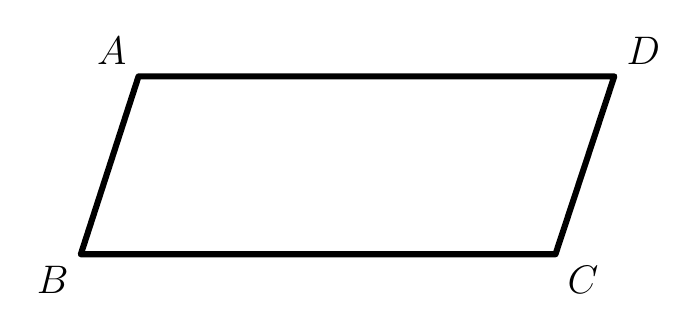
\begin{tikzpicture}[line join=round, line width=2.2pt]
  % Vertices (pixel coords converted with s = 0.019139, centred on ink bbox)
  \coordinate (A) at (-2.667,1.139);
  \coordinate (B) at (-3.400,-1.120);
  \coordinate (C) at (2.628,-1.120);
  \coordinate (D) at (3.375,1.139);

  % Sides
  \draw (A) -- (B) -- (C) -- (D) -- cycle;

  % Labels outside the corners
  \node[above left, font=\fontsize{15.5}{18.6}\selectfont] at (A) {$A$};
  \node[below left, font=\fontsize{15.5}{18.6}\selectfont] at (B) {$B$};
  \node[below right, font=\fontsize{15.5}{18.6}\selectfont] at (C) {$C$};
  \node[above right, font=\fontsize{15.5}{18.6}\selectfont] at (D) {$D$};
\end{tikzpicture}
\end{document}